\documentclass[a4paper,png]{article}
\usepackage[utf8]{inputenc}
\usepackage[L7x]{fontenc}
\usepackage[lithuanian]{babel}
\usepackage{lmodern}
\usepackage{amsmath}
\usepackage[top=2cm, bottom=2cm, left=1cm, right=1cm, footskip=1cm, a4paper]{geometry}
\usepackage{hyperref}
\usepackage{verbatim}
\usepackage{tasks}
\usepackage{mdframed}
\usepackage{tabularx}
\usepackage{xcolor}
\usepackage{indentfirst}
\usepackage{graphicx}

%DEFINITION
\newcommand{\fillup}[1]{\begin{tabular}{m{0.95\linewidth}m{0.05\linewidth}}#1 & \phantom{$\begin{array}{c}.\\.\end{array}$}\end{tabular}}
\newcommand{\learn}[7]{
\begin{tabular}{||p{0.48\textwidth}|p{0.48\textwidth}||}
\multicolumn{2}{c}{#1}\\
\hline \hline
\textcolor{black!50!white}{\fbox{Procedūra (tai, ką reikės atlikti)}}\par \fillup{#2} & \textcolor{black!50!white}{\fbox{Sąvoka (kas tai yra?)}}\par \fillup{#3} \\ \hline 
\textcolor{black!50!white}{\fbox{Procedūros atlikimas (kaip gauti rezultatą?)}}\par \fillup{#4} & \textcolor{black!50!white}{\fbox{Perkeltinė prasmė (su kuo siejame skaičius/simbolius?)}}\par \fillup{#5} \\ \hline 
\textcolor{black!50!white}{\fbox{Vaizdinys (kaip panaudoti perkeltinę prasmę?)}}\par \fillup{#6} & \textcolor{black!50!white}{\fbox{Paaiškinimas (ką atlikome vaizdinyje?)}} \par \fillup{#7}
\\\hline \hline
\end{tabular}}

%USE
\begin{document}
\section*{Naujas darbo pamokose modelis}
Kaip žinia, mokyklinis matematikos kursas yra orientuotas tik į mokinių gebėjimą atlikti kuo daugiau procedūrų. Šios procedūros su kiekvienu matematikos vadovėlių perleidimu yra vis iš naujo perstruktūrizuojamos, tačiau mokinio akimis šie  mokyklinio kurso pakeitimai tebūtų tik nežymūs pakitimai iš vieno milžiniško dydžio tarpusavyje nesusijusių taisyklių rinkinio į kitą. Toks procedūrinio mąstymo ugdymas moksleivius atveda į aklavietę, kuomet medžiagos yra per daug, o būdų jai suvokti ir įsiminti moksleiviai nežino. Produktyvūs matematikos įsiminimo būdai reikalauja pažangesnio kalbos ir vaizduotės išnaudojimo. Juos galime laikyti tiesiog gebėjimu mąstyti matematiškai. Gabesnieji moksleiviai bei mokytojai gebėdami mąstyti matematiškai matematikos pamokų turinį ne tik išmoksta, bet ir supranta. Tačiau keblumų kyla, kai reikia tai, ką supranta, paaiškinti silpnesniesiems. Mano požiūriu matematinių procedūrų paaiškinimas reikalauja mąstymo procesų išmanymo, detalaus plano, kodėl viena ar kita taisyklė daliai moksleivių gali būti nesuprantama, ir būti toks, kad reikėtų įdėti kuo mažiau pastangų norint jį prisiminti būsimose pamokose. 

Čia pateiksiu aiškinimo planą, kuriame atsispindi, kaip galima nagrinėti uždavinius, kad šis nagrinėjimas neapsiribotų greit atmintyje išblėstančia žingsnių seka, o būtų suteikiantis matematinio mąstymo (t.y. vaizduotės ir kalbos išnaudojimo), būtino, kad žingsnių seka taptų atmintyje neišblėstanti.

Viena iš didesnių problemų bandant aiškintis ne atliekamų aritmetinių ir algebrinių veiksmų procedūras, o jų prasmę, yra ta, jog moksleiviams toks aiškinimosi būdas yra pakankamai nauja medžiaga, atspindinti nemažą kiekį galvoje nespėjusių struktūrizuotis idėjų. Dėl šios priežasties moksleiviams yra sunku atrinkti, kurios iš idėjų yra įsimintinos, o kurios yra išsamprotaujamos savo pastangomis ir padedančios įsiminti kitas idėjas. Tai nulemia didelės dalies svarbios informacijos, kurios reikės kitokiai arba panašiai medžiagai suprasti, išblėsimą atmintyje. Atkreipkime dėmesį, jog minėtų idėjų aptarimas užtrunka. Pakartotinai aptariant medžiagą su moksleiviais patiriami dideli laiko nuostoliai, tad gali nesigauti suspėti kartu su mokylinės programos tempu. Siekiant sumažinti šiuos nuostolius siūlau procedūrų paaiškinimą užsirašyti tam tikra lentelės forma, prie kurios sprendžiant vis sunkesnius uždavinius būtų galima iš naujo sugrįžti, tačiau dėl to nepatirti didelių laiko nuostolių. Reikalavimas: tai, ką užsirašėme moksleiviui turi būti prieinama kiekvieną pamoką. Štai, kaip atrodo lentelė:
\newline \newline 
\noindent
\learn{{\fbox{\phantom{$\frac{2}{3}+\frac{3}{4}+\frac{4}{5}$}}}}
{}{}
{}{}
{}{}
\newline

\renewcommand{\fillup}[1]{\begin{tabular}{m{0.95\linewidth}m{0.05\linewidth}}#1 & \phantom{$\begin{array}{c}.\\.\\.\\.\\.\end{array}$}\end{tabular}}

Lentelės pildymo idėjos tokios: 
\begin{enumerate}
\item Užsirašome, kokią procedūrą reikės taikyti sprendžiant uždavinį, koks būtų jos atlikimas mokykloje ir įvardijame reiškinį, kurį apskaičiavome. Taip lavėja ne tik procedūrų atlikimo įgūdžiai, bet ir kalba, reikalinga mąstyti matematiškai.
\item Aš pasiūlau paaiškinimą, kokią prasmę galime suteikti uždavinuke naudojamiems skaičiams ir veiksmams. Ši prasmė yra pagrindinė informacija, kurią reikia atgaminti sprendžiant panašius ar sunkesnius uždavinius.
\item Kartu su moksleiviu sugalvojame, kokia iliustracija tiktų pavaizduoti šią prasmę. Vaizdinys - tai antras dalykas (be kalbos), būtinas mąstyti matematiškai.
\item Išsiaiškiname, kaip remiantis iliustracija būtų galime paaiškinti sprendimą, kurį atliktume mokykloje.
\item Pildydami lentelėse išsprendžiame dar kelis panašaus pobūdžio uždavinukus, kritiškai įvertiname, kaip jų idėjos siejasi su ankstesniais lentelėse spręstais uždaviniais, įveikiame sunkiąsias vietas.
\item Toks suformuotas kritinis vertinimas ir sunkiųjų vietų išsiaiškinimas gali būti vadinamas žinių užtvirtinimu savo patirtimi. Jis reikalingas ir tam, kad mąstymas sprendžiant uždavinį taptų pakankamai matematišku, ir tam, kad sprendimo procedūra būtų atmintyje neišblėstanti.
\end{enumerate}

\newpage
\noindent
\learn{{\Huge{\fbox{\phantom{$\frac{2}{3}+\frac{3}{4}+\frac{4}{5}$}}}}}
{}{}
{}{}
{}{}
\newline \newline \newline%%%
\noindent
\learn{{\Huge{\fbox{\phantom{$\frac{2}{3}+\frac{3}{4}+\frac{4}{5}$}}}}}
{}{}
{}{}
{}{}
\newline \newline \newline%%%
\noindent
\learn{{\Huge{\fbox{$\frac{2}{3}+\frac{3}{4}$}}}}
{Dviejų trupmenų sudėtis}{Dviejų trečiųjų ir trijų ketvirtųjų suma}
{{\Large{$\frac{2}{3}+\frac{3}{4}=\frac{8}{12}+\frac{9}{12}=\frac{8+9}{12}=\frac{17}{12}=1\frac{5}{12}$}}}{Stačiakampio dalys}
{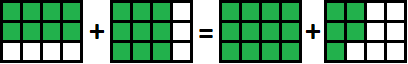
\includegraphics[width=0.47\textwidth]{cdenom.png}}{Sudėję 2 trečiąsias stačiakampio su 3 ketvirtosiomis stačiakampio gauname vieną pilną stačiakampį ir 5 dvyliktąsias stačiakampio}
\newline \newline\newline%%%
\learn{{\Huge{\fbox{$-(x-y)$}}}}
{Atskliaudimas turint prieš skliaustus minusą}{Skaičius, neigiamas $x$ ir $y$ skirtumui}
{$-(x-y)=-x+y$}{1) Minusą siejame su poslinkio krypties keitimu;\par 2) Kintamąjį siejame su poslinkiu pirmyn;\par 3) \textbf{Pastaba}: pliuso ir minuso ženklai, rašomi prie kintamųjų, taip pat žymi, kad poslinkiai atliekami vienas po kito}
{$\underbrace{
\includegraphics[width=0.2\textwidth]{add_vec.png}}_{\text{\textbf{\textit{apkeisti suminio poslinkio kryptį}}}} 
\includegraphics[width=0.21\textwidth]{added_vec.png}$}{Apkeitę poslinkio, gauto sudėjus poslinkus $x$ pirmyn ir $y$ atgal, kryptį, gauname tą patį, ką ir sudėję atitinkamus priešingų krypčių poslinkius}
\newline \newline \newline%%%
\learn{{\Huge{\fbox{49\% skaičiaus 16}}}}
{Procentinės dalies radimas}{49\% skaičiaus 16}
{{\Large{$\text{49\% skaičiaus 16}=49\times 0,16=7,84$}}}{Procentas atitinka šimtąją dalį \par Skaičius atitinka didelio kvadrato plotą}
{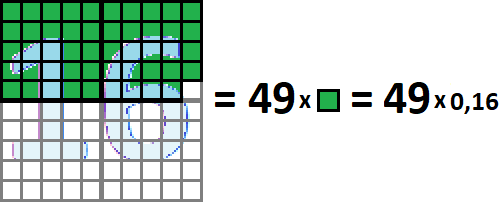
\includegraphics[width=0.46\textwidth]{percentage.png}}{Norėdami rasti 49\% kvadrato, kurio plotas 16, iš pradžių randame, koks yra kvadrato šimtadalio plotas, o po to randame, koks yra 49 šimtadalių plotas}
\newline \newline \newline%%%
\learn{{\Huge{\fbox{$\sqrt{50}$}}}}
{Šaknies traukimas iš sudėtinio skaičiaus}{Šaknis iš 50}
{{\Large{$\sqrt{50}=\sqrt{5\times 5\times 2}=5\sqrt{2}$}}}{Šaknis iš duoto skaičiaus yra apibrėžiama kaip toks teigiamas skaičius, kurio kvadratas lygus duotam skaičiui;\par Skaičių siejame su pirminių daugiklių, įeinančių į jo skaidinį dauginamaisiais, rinkiniu (jį apjungia daugybos veiksmas); \par Šaknies traukimą siejame su šio rinkinio skėlimu į dvi lygias dalis}
{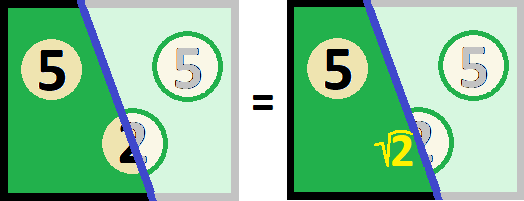
\includegraphics[width=0.46\textwidth]{rooting.png}}{Norėdami rasti $\sqrt{50}$, skaičių 50 įsivaizduojame kaip daugiklių, esančių sandaugoje $5\times 5\times 2$ rinkinį, o šaknį iš 50 kaip šio rinkinio pusę. Skeldami penketų porą pusiau, gauname vieną penketą. Vieno dvejeto perskelti į pusę daikto negalime, nes negalime suvokti sandaugos, kurioje būtų pusė daugiklio. Todėl dvejeto skėlimo proceso, neturinčio suvokiamo rezultato, nevykdome, o vietoj to paliekame skaičių $\sqrt 2$, kuris atitinka ieškotą daugiklį, nes tenkina $\sqrt 2 \times \sqrt 2 = 2$}
\newline \newline \newline%%%
\learn{{\Huge{\fbox{$7\times 4$}}}}
{Dviejų (natūraliųjų) skaičių daugyba}{Skaičių 4 ir 7 sandauga}
{$\Huge{4\times 7=28}$\\ $\left\{\begin{array}{l}\text{Pagal daugybos lentelę, jei tai vienženkliai skaičiai;}\\ \text{Dauginant stulpeliu, kitais atvejais.}\end{array}\right.$}{1) Pirmasis daugiklis - eilučių kiekis; \par 2) Antrasis daugiklis - kvadratėlių kiekis eilutėje;\par \par 3) Sandauga - kiek kvadratėlių iš viso?}
{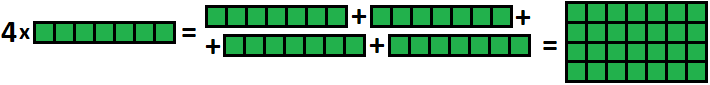
\includegraphics[width=0.46\textwidth]{mul47.png}}{Daugyba $4\times 7$ atitinka, kiek mažų kvadratėlių yra stačiakampyje $4\times 7$. Šį kiekį galime rasti sudėdami 4 kvadratėlių eilutes po 7 kvadratėlius}
\newline \newline \newline%%%
\learn{{\Huge{\fbox{$(x-y)(x+y)=?$}}}}
{dviejų skaičių skirtumo ir sumos daugyba}{Skaičių $x$ ir $y$ skirtumo ir sumos sandauga}
{$\Huge{(x-y)(x+y)=x^2-y^2}$\\ (tai yra kvadratų skirtumo formulė)}{1) Dėmenys, įeinantys į pirmą daugiklį atitinka tai, kas sudaro stačiakampio ilgį; \par 2) Dėmenys, įeinantys į antrą daugiklį atitinka tai, kas sudaro stačiakampio plotį \par 3) Sandauga atitinka stačiakampio plotą}
{}{Norėdami suskaičiuoti viso stačiakampio plotą sudedame jo atskirų dalių ploto atitikmenis.}
\newpage 
\section*{Pastabos apie pratimus}
\section{Pratimas $(a+b)^2=a^2+2ab+b^2$}
\fbox{Mantas, 6kl.}
\begin{itemize} 
\item Pirmiausia turėdamas brėžinį Mantas nesuvokia, kas yra $a$ ir $b$. Aš parodau, kad tai brėžinyje matomų atkarpų ilgiai.
\item Mantas suvokia, jog $a+b$ tuomet atitinka kvadrato kraštinės ilgį, tačiau negeba apibūdinti $a$ ir $b$ prasmės (atkarpų, gautų atlikus kvadrato kraštinės padalijimą, ilgiai)
\item Faziniai sunkumai: $(a+b)^2$ neturi prasmės, nors $3^2$, kai 3 yra kvadrato kraštinė, turi.
\item Kalbiniai sunkumai: sunku perskaityti reiškinį $x^2+y^2+(x-y)^2$ naudojant terminus ,,suma ir kvadratas''. Mantas bando nusakyti $(x-y)^2$. Sako: $x$ ir $y$ kvadratu skirtumas.
\end{itemize}
\section{Trupmenos 24/48 prastinimas}
\fbox{Mantas, 6kl.}
\begin{itemize} 
\item Mantui neaišku, ką daryti, kai atlikus prastinimą $\frac{2\cdot 2\cdot 2\cdot 3}{2 \cdot 2\cdot 2\cdot 2\cdot 3}$ skaitiklyje nieko nelieka. Iš to išplaukia, jog jam reikėjo būti mačius ,,daugybos lentą''.
\item Kortelė 2 daugybos stale yra pakeičiama į korteles 2 ir 1. Dabar Mantas galvoja, jog suprato visą sprendimą.
\item Manto manymas apgaulingas. Iš tiesų, jam aišku, kodėl $\boxed{7:2=3,5} \Rightarrow\boxed{3,5 \times 2=7}$. Atvejis $\boxed{7:2:4=\frac{7}{8}} \Rightarrow$ $\boxed{\frac{7}{8} \times 4 \times 2=7}$ aiškus mažiau. Jei nariuose yra šaknys, aiškumas išnyksta visiškai. Taigi, jam reikėjo būti mačius veiksmų ,,apgrežiamumą''. Stebėti sunkumai yra taip pat faziniai.
\item Veiksmo ,,Apgrežiamume''  dalyvaujantys loginiai elementai yra panašūs, kaip ir ,,uždavinio sprendime iš kito galo''. Daviau Mantui pabandyti uždavinį ,,Aš sugalvoju skaičių. Trissyk jį padauginu iš 2 ir pridedu 1. Gaunu 47. Koks tai skaičius?
\end{itemize}
\section{Reiškinio $x^2-5x+6$ išskaidymas dauginamaisiais}
\fbox{Tomas, 9kl.}
\begin{itemize}
\item Tampa akivaizdu, jog atspėjimas tokių skaičių, kurių suma yra 5, o sandauga 6 yra grindžiamas tik tuo, kad tokios taisyklės parašytos vadovėlyje.
\item Nors vadovėlyje yra pratimas, kuriame reikia pasipraktikuoti užrašyti keleto teig. ir neig. skaičių sandaugas sveikais daugikliais, Tomas nori padaryti jį greičiau ir atsisako patyrinėti, kaip palaipsniui keičiantis daugikliams keičiasi jų suma (tiksliau palieka šią eigą namuose)
\item Tomas atsisako pats atlikti ženklų keitimus daugikliuose, daugiklių eilės apgręžimą ir abudu kartu.
\item Tomas pusę uždavinių su teig. - neig. skaičių veiksmais atlieka neteisingai, nes naudojasi kalkuliatoriumi, neturinčio skaičiaus užminusavimo funkcijos ir atsisako panaudoti teig. - neig. skaičių įprasminimą.
\item Vėlesniame kontekste Tomui neaišku, kad skaidant $x^2-5x+6$, reikia pradėti nuo 6 skaidymo daugikliais ir išrinkti pora tokių daugiklių, kad jų suma yra 5.  Problema matomai psichologinė: atsisakymas suprasti => atsisakymas įgyti pasitikėjimo => negalėjimas įgyti žinių, būtinų spręsti kitam uždaviniui.
\end{itemize}
\section{Taisyklė $\frac{a^n}{b^n}=\left(\frac{a}{b}\right)^n$}
\fbox{Elena, 7kl.}
\begin{itemize}
\item Dalybos ir daugybos ryšio suvokimas Elenai naujas. Taip pat ir perprasminimas, kad kortelių atėmimą iš nulio reikėtų, apkeisti su samprotavimais  ,,Jei lentoje pašaliname daugiklį, tai reiškia rezultatą sumažiname tiek kartų, koks buvo daugiklis. Tai yra tas pats, kas lentą papildžius tuo pačiu dalikliu vėl tiek pat kartų sumažinti rezultatą. Vadinasi atmesti daugiklį reiškia papildyti tuo pačiu dalikliu. Štai kodėl daugyba atvirkščia dalybai.''
\item Kalbiniai sunkumai: Trūksta pajutimo, kas vaizduojama kairėje lygybės pusėje ir kas dešinėje.
\item Kalbiniai sunkumai: analogija su $(-2)^7=-2^7$. Tai parodo, kodėl taip svarbu užrašinėti pilnus reiškinių pavadinimus. 
\end{itemize}
\end{document}